\section{Spécification du Système}
Cette partie du cahier de charge présentera les trois axes principaux du développement de ifind.
\begin{itemize}
 \item Architecture du système.
 \item Charges du système.
 \item Modèles dy système.
\end{itemize}

\subsection{Architecture du Système}
Ce paragraphe présente un point du vue haut niveau de l'architecture préconisée du système et la distribution de fonctionnalités à travers 
les modules du système.

Notre système ce compose de trois sous-système :
\begin{itemize}
 \item Moteur de recherche : Architecture Model View Controler
 \item Moteur d'indexation : Deamon
 \item Base de donnée indexée : Architecture en couche : PostgreSQL + surcouche de gestion de la base de donnée : Hibernate
\end{itemize}

\subsubsection{Architecture du Moteur de recherche}

\paragraph{BNF}
Nous avons défini une syntaxe et à fortiori, une grammaire sous forme BNF.

Grammaire (BNF) :\\
% \begin{tabular}{r c l}
% query &$\rightarrow$ & word { -or word } [options]\\
% query &$\rightarrow$ & word { word } [options] \\
% 	 
% options&$\rightarrow$ &-e word {word}\\
% word   &$\rightarrow$ &char*\\
% char   &$\rightarrow$ & [a-z A-Z 0-9 à é è ë ä ù ï ç]\\ 
% \end{tabular}

\begin{tabular}{p{1.5cm} p{0.5cm} p{9cm} }
& & \\
\textbf{char} & $\equiv$ & [:alnum:]\\
\textbf{word} & $\equiv$ & $\textbf{char}^+$\\
\textit{query} & ::= & \textbf{word} \textit{\{} \textbf{-or} \textbf{word} \textit{\}} \textit{[} \textit{options} \textit{]}\\
& | & \textbf{word} \textit{\{} \textbf{word} \textit{\}} \textit{[} \textit{options} \textit{]}\\
\textit{options} & ::= & \textbf{-e} \textbf{word} \textit{\{} \textbf{word} \textit{\}}\\
\end{tabular}

Par la suite, nous avons défini plusieurs types abstraits de données permettant de modéliser la grammaire.
Un type a forcément une ou plusieurs opérations de construction. 
Chaque type peut présenter des fonctions d'accès et de test ainsi que des constantes.

\paragraph{Type de données abstraites}
En effet, nous avons définit 6 types tels que :

\begin{tabular}{r l}
%\textbf{Type : operateur} & \\
%constantes :& plus, OR et Exclu : operateur
% note (isabelle) La présence des types [conj] et [disj] rend la constante [operateur] inutile.

\textbf{Type : requête} & \\
_construction :& cons-requete-word : word $\rightarrow$ requête\\
& cons-requete-word-options : word * options $\rightarrow$ requête\\ 
& cons-requete-conj : conj $\rightarrow$ requête\\
& cons-requete-conj-options : conj * options $\rightarrow$ requête\\
& cons-requete-disj : disj $\rightarrow$ requête\\
& cons-requete-disj-options : disj * options $\rightarrow$ requête\\
_test :& est-word : requête $\rightarrow$ bool\\
& est-conj : requête $\rightarrow$ bool\\
& est-disj : requête $\rightarrow$ bool\\
& a-options : requête $\rightarrow$ bool\\
% est-valide : requête $\rightarrow$ bool\\
% note (isabelle) une requête qui est construite est par définition valide (sauf erreur de ma part), donc ce test est inutile.
_accès :& get-word : requête $\rightarrow$ word\\
& get-conj : requête $\rightarrow$ conj\\
& get-disj : requête $\rightarrow$ disj\\
& get-options : requête $\rightarrow$ options\\
\end{tabular}

\paragraph{}
On garde get-conj() si est conj : get-word() puis recherche conjonction et
get-disj() si est disj : get-word() puis recherche disjonction.
\paragraph{}

\begin{tabular}{r l}
\textbf{Type : conj} &\\
_construction :& cons-conj : word * conj $\rightarrow$ conj\\
& cons-conj-simple : word * word $\rightarrow$ conj\\
_test :& est-conj : conj $\rightarrow$ bool\\
_accès :& get-head : conj $\rightarrow$ word\\
& get-tail : conj $\rightarrow$ conj\\
& \\

\textbf{Type : disj}&\\
_construction :& cons-disj : word * disj $\rightarrow$ disj\\
& cons-disj-simple : word * word $\rightarrow$ disj\\
& accès : getDisj()\\
& \\

\textbf{Type : word}&\\ 
_construction :& cons_word : string $\rightarrow$ word\\
_accès :& get-word : word $\rightarrow$ string\\
& \\

\textbf{Type : options}&\\
_construction :& cons-options : word $\rightarrow$ options\\
& cons-options-simple : word * word $\rightarrow$ options\\
_test :& est-options : options $\rightarrow$ bool\\
_accès :& get-head : options $\rightarrow$ word\\
& get-tail : options $\rightarrow$ options
\end{tabular}


Model :

View : GUI

Controler : search-engine-core
\begin{center}
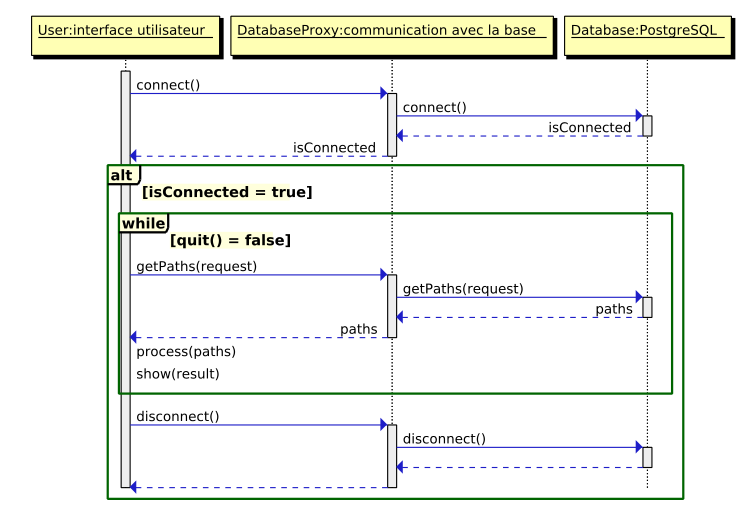
\includegraphics[scale=0.5]{seqmrbi.png}
\end{center}


\subsubsection{Architecture du moteur d'indexation}
Il s'agit juste d'un démon parametrable qui construit en premier temps une base d'indexation 
ensuite il communique avec celle-ci à l'aide d'un protocole de communication par socket.

La communication entre la base d'indexation et le moteur d'indexation a pour but la mis-à-jour de la BD.

\subsubsection{Architecture de la base d'indexation}
La base d'indexation est une base de donnée PostgreSQL, en un premier temps, qui permettra au moteur de recherche 
de retrouver ce qu'il cherche.

\begin{center}
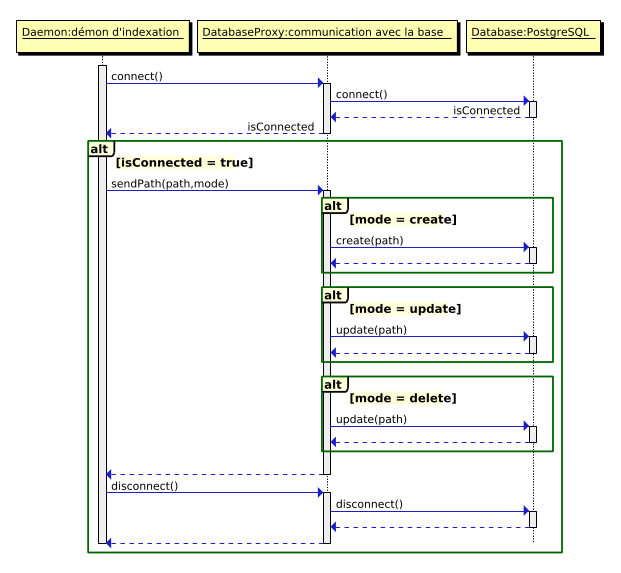
\includegraphics[scale=0.5]{seqdbi.png}
\end{center}

Le modèle conceptuel de données (MCD) de la base de données est le suivant :
\begin{center}
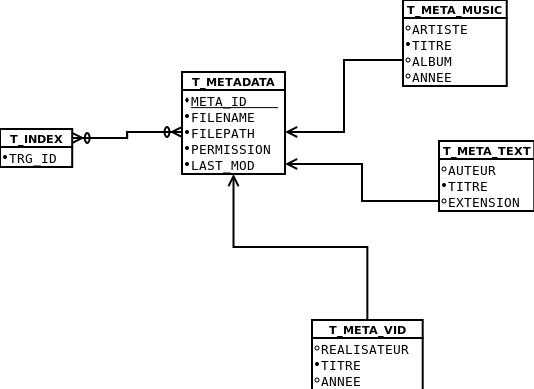
\includegraphics[scale=0.7]{mcd.png}
\end{center}


\subsection{Charges du Système}
Ce paragraphe décrit les charges fonctionnelles du système en détail et d'autres charges non fonctionnelles : 
\begin{itemize}
 \item interface
 \item autres...
\end{itemize}

\subsection{Modèles du système}
Ce paragraphe décrit les divers modèles du système ainsi que leurs relations entre composantes du système et de son environnement.

\subsubsection{Modèle de communication}
le module de BD crée deux sockets Server :\\
L’instanciation de ces sockets doit se faire avec les informations lues à partir des fichier config-sample-Deamon.XML et config-sample-MoteurR.

On définit tout d'abord la socket entre la base d'indexation et le moteur de recherche. Le socket reste en écoute 
des requêtes en provenance du moteur de recherche, une requête est un fichier XML générée suite à une seule et unique recherche pour 
cela on doit impérativement ajouter un identifiant dans la DTD au retour. Chaque réponse génère un seul fichier 
XML qui sera envoyé au moteur de recherche on peut facilement retrouver l'ordre grâce au ID de chaque requête. 

On distingue un cas particulier : par exemple l'envoie des résultats en morceaux , quand la recherche prend éventuellement du temps. 
Là aussi il faut ajouter des informations supplémentaires dans la DTD pour qu'on puisse rendre possible ce genre d'opérations.

On définit ensuite la socket entre la base d'indexation et le moteur d'indexation. Le socket reste en écoute de nouvelle information capturée par le démon
(Daemon). Chacun peut choisir sa politique de mise à jour ( envoie du fichier XML chaque 20 min par ex etc .) 
On doit se mettre d'accord sur le format d'échange pour ces deux modules. 

\paragraph{Remarques :} J'ai choisi les ports de façon arbitraires il y a 3 ports le premier et celui par défaut 
si jamais ce port n'est pas libre ont basculera vers le 2e etc. 

\paragraph{Remarque 2 :} La DTD bd2M. n'est pas encore assez riche pour gérer une recherche dont le nombre 
de mots-clés et supérieur à 1 comme on l'a vu au TD. Il faut prendre en considération tous les cas possibles, exemple :
mot1 ou mot2 , mot1 et mot2, etc. 

Je propose qu'on rajoute de nouveaux éléments en dehors de la balise search qui concerne la manière dont on va l'interpréter.